\documentclass[xcolor=table]{beamer}

\uselanguage{English}
\languagepath{English}
\usetheme{HongKong}
\useinnertheme{rounded}
\usepackage{color, colortbl}
\usepackage{tcolorbox}
\usepackage{multirow} 
\usepackage{textcomp}
\usepackage{siunitx}
\usepackage{tikz}
\usepackage[utf8]{inputenc}
\usepackage[safe]{tipa}
\usepackage{array}
\usepackage{hhline}
\usepackage{pbox}

\usepackage{etoolbox}

\usepackage{algorithm,algorithmic}
%\usepackage[noend]{algpseudocode}

\tikzset{rndblock/.style={rounded corners,rectangle,draw,outer sep=0pt}}
\newcommand{\tframed}[2][]{\tikz[baseline=0.1pt]\vspace{0.1cm}\node[rndblock,minimum height=1.5em,#1] (m) {#2} ;}
\newcommand{\hilight}[1]{\textbf{\tframed[blue,fill=blue!10]{#1}}}
\newcommand{\whilight}[1]{\textbf{\tframed[purple,fill=purple!10]{#1}}}

\newcommand{\sP}{\hspace{1pt}}
\newcommand{\mP}{\hspace{3pt}}
\newcommand{\bP}{\hspace{6pt}}
\newcommand{\BP}{\hspace{12pt}}


\newcolumntype{L}[1]{>{\raggedleft\let\newline\\\arraybackslash\hspace{0pt}}m{#1}}

%\newcommand{\hilight}[1]{\colorbox{white}{#1}}

%==============================================================================================================

\setbeamertemplate{navigation symbols}{}
\setbeamertemplate{items}[ball] 
\setbeamertemplate{blocks}[rounded][shadow=true,width=.7\textwidth] 

\setbeamercolor{myBlueBox} {bg=blendedblue, fg=white}
\setbeamercolor{myGrayBox} {bg=blendedgray, fg=black}

\definecolor{darksalmon}{RGB}{233,150,122}
\definecolor{blendedblue}{rgb}{0.137,0.466,0.741}
\definecolor{blendedgray}{rgb}{0.838,0.833,0.833}
\definecolor{blendedpurple}{RGB}{75,20,130}
\definecolor{tgray}{rgb}{0.211, 0.211,0.244}
\definecolor{darkgray}{rgb}{0.450,0.450,0.450}
\definecolor{maroon}{rgb}{0.665, 0.142, 0.142}
\definecolor{ngreen}{rgb}{0.000,0.500,0.000}

\newcolumntype{g}{>{\columncolor{tgray}}S[tabformat=2.2]}

\newenvironment<>{varblock}[2][\textwidth]{%
\vspace*{-20pt}
	  \setlength{\textwidth}{#1}
	  \begin{actionenv}#3%
	    \def\insertblocktitle{#2}%
	    \par%
	    \usebeamertemplate{block begin}}
	  {\par%
	    \usebeamertemplate{block end}%
	  \end{actionenv}
\vspace*{-20pt}
}


%\setbeamertemplate{itemize item}{$\blacktriangleright$}
\setbeamertemplate{itemize subitem}{$\ast$}
\setbeamerfont{itemize/enumerate subbody}{size=\footnotesize} 							%to set the body size
%\setbeamertemplate{itemize subitem}{\tiny\raise1.25pt\hbox{\donotcoloroutermaths$\blacktriangleright$}}  	%to set the symbol size


%==============================================================================================================

\title{Combining lexical and prosodic features for automatic detection of sentence modality in French}
\author[Luiza Orosanu, Denis Jouvet]
{
\vskip0.3cm \textbf{Luiza Orosanu, Denis Jouvet}
\vskip0.45cm  INRIA-Loria, Nancy, France  \\
\vskip0.15cm Multispeech Team\vspace{-1cm}
}
\date{}

\AtBeginSection[]
{
  \begin{frame}
	\thispagestyle{empty}
   	\frametitle{Summary}
	\tableofcontents[currentsection, hideothersubsections,sectionstyle=show/shaded, subsectionstyle=show/shaded/hide] 	%subsectionstyle=show/shaded,currentsection,subsections, currentsubsection]
  \end{frame}
}


\AtBeginSubsection[]
{
  \begin{frame}
	\thispagestyle{empty}
   	\frametitle{Summary}
	\tableofcontents[currentsubsection, hideothersubsections,sectionstyle=show/shaded, subsectionstyle=show/shaded/hide] 	
  \end{frame}
}


\newcommand{\firstslide}{%
	\begin{frame}
	\hfill
	\thispagestyle{empty}
	\titlepage
	\end{frame}
}

%==============================================================================================================
\begin{document}
\renewcommand{\inserttotalframenumber}{18}

%==============================================================================================================
\firstslide


%==============================================================================================================
\section{Context and approach} 
\begin{frame}[t]{Context}
\setcounter{framenumber}{1}

{\scriptsize \textbf{\color{purple}Objective} : state from the automatic transcription if the sentence \\\hskip12ex is a question or a statement }

\bigskip
\begin{center}
\vskip-3ex
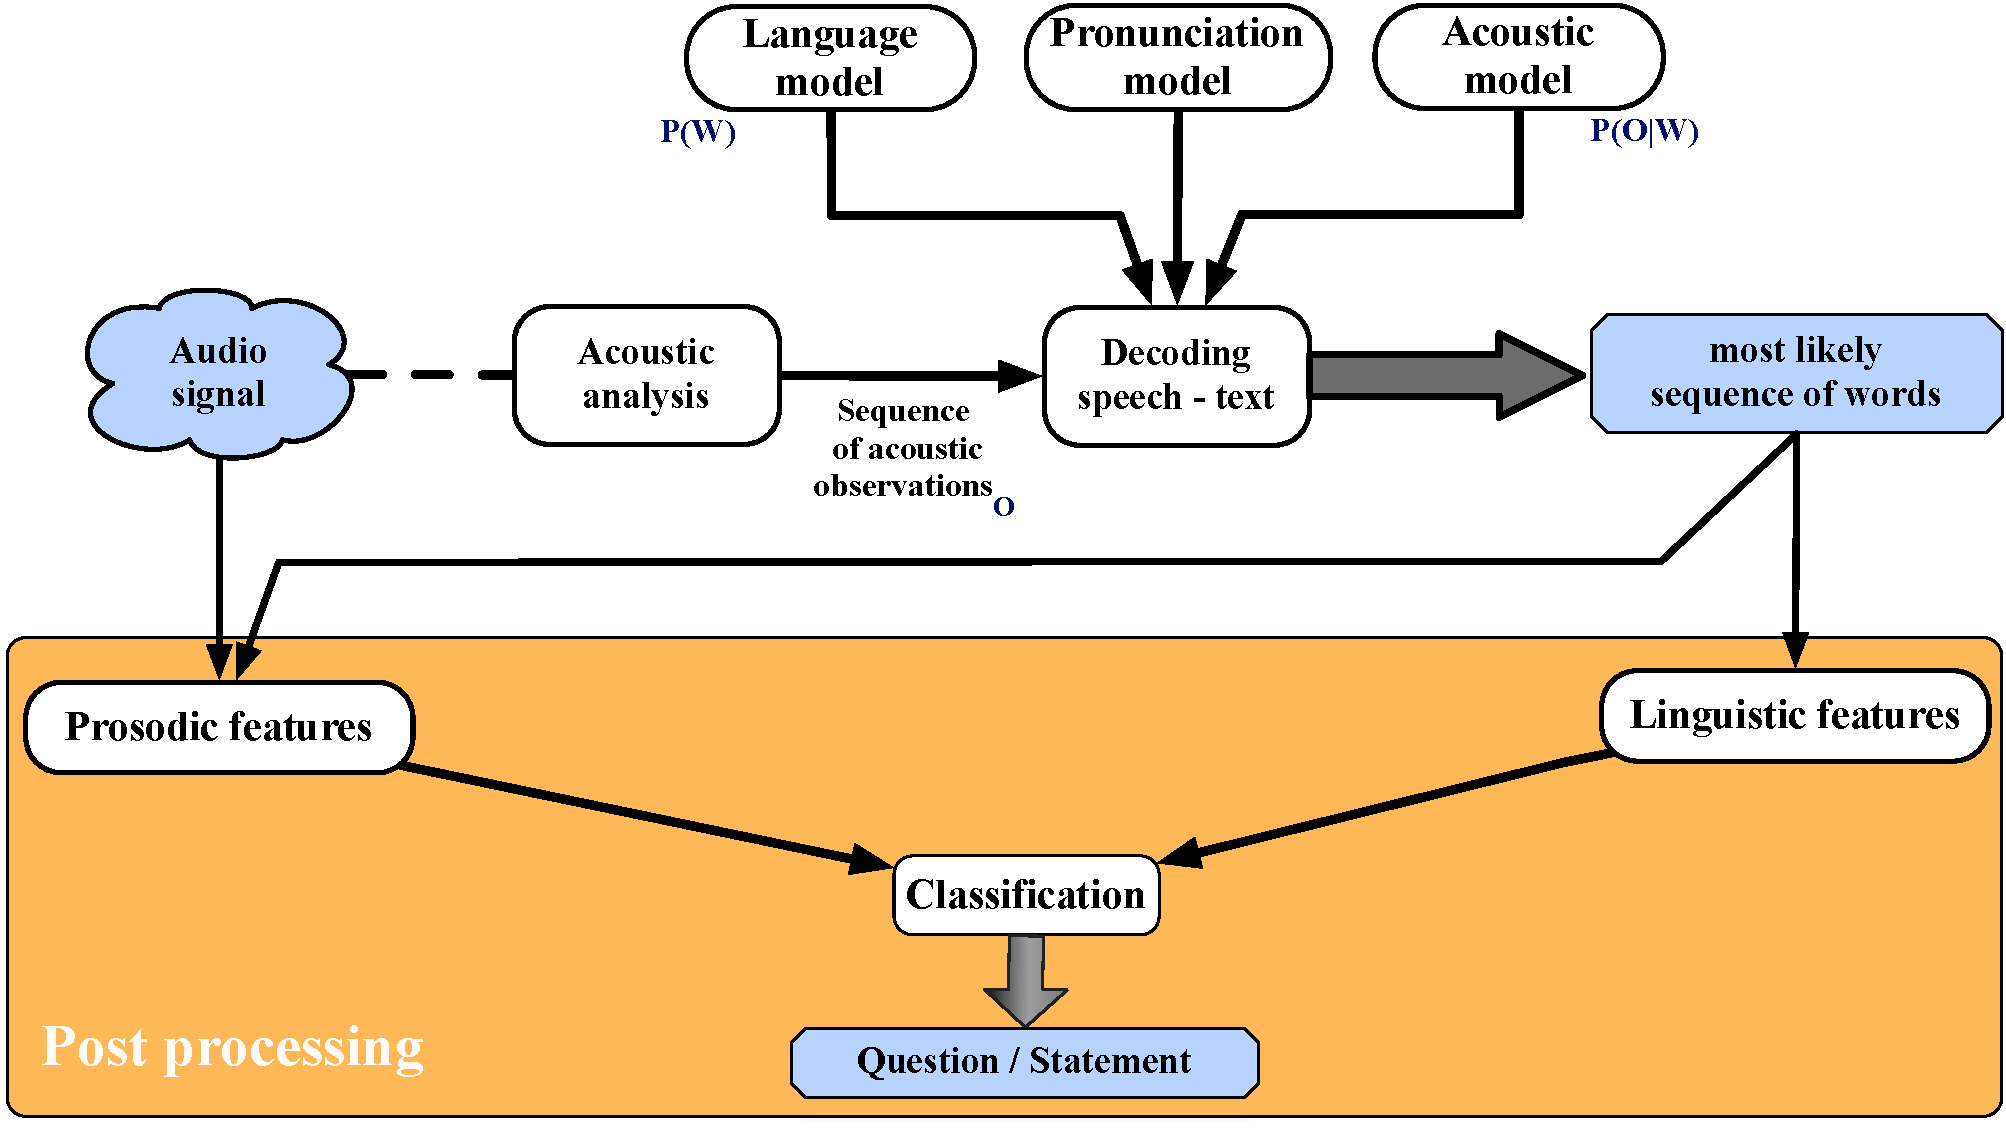
\includegraphics[scale=0.32]{Image/picture/QD_last_en.pdf}
\end{center}


\end{frame}


%==============================================================================================================
\begin{frame}[t]{Approach}

\begin{itemize}

\vskip-1ex
\item \textbf{\color{purple}prosodic classifier} : uses the intonation
	
	\vskip0.1ex\hskip0.8ex {\scriptsize {\color{blendedblue}$\rightarrow$} sentences perceived as questions through the intonation}
		
		\vskip0.1ex
		\begin{center}
		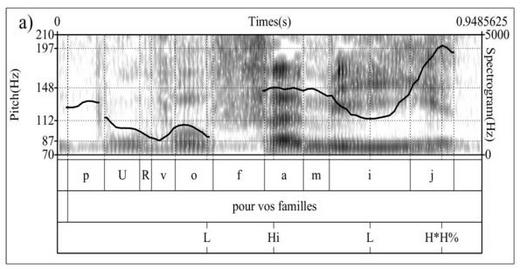
\includegraphics[scale=0.3]{Image/picture/prosodie}
		\end{center}
	
\vspace*{0.1ex}
\item \textbf{\color{purple}linguistic classifier} : uses the linguistic information

	\vskip0.1ex\hskip0.8ex {\scriptsize {\color{blendedblue}$\rightarrow$} sentences perceived as questions through the interrogative forms}
		
		\vskip0.4ex\hskip5ex {\scriptsize {\color{blendedblue}$\ast$} qu'est ce qu'on doit comprendre ? \\\vskip-1ex\hskip15ex \textit{\color{darkgray}($\rightarrow$ what should we understand?)}}
		\vskip1.1ex\hskip5ex {\scriptsize {\color{blendedblue}$\ast$} est ce que vous souhaitez une confrontation ? \\\vskip-1ex\hskip15ex \textit{\color{darkgray}($\rightarrow$ do you want a confrontation?)}}
		
\vskip1.5ex
\item \textbf{\color{purple}combined classifier} : uses both types of information
\end{itemize}

\end{frame}


%==============================================================================================================
\begin{frame}[t]{Approach}

\begin{itemize}

\vskip10ex
\item evaluate classifier on \textbf{\color{purple}manual transcriptions}
	\vskip1ex\hskip3ex {\color{blendedblue}$\rightarrow$} ideal conditions - 0\% word error rate

\vskip5ex
\item evaluate classifier on \textbf{\color{purple}automatic transcriptions}
	\vskip1ex\hskip3ex {\color{blendedblue}$\rightarrow$} real conditions - 26\% word error rate

\end{itemize}

\end{frame}



%==============================================================================================================
\section{Prosodic and linguistic features}
\begin{frame}[t]{Prosodic features (\#10)}
\setcounter{framenumber}{4}

\vskip1.2cm
\begin{itemize}

\item generally, a question has a final rising pitch
	
\bigskip
\item we compute 10 prosodic features that take into account 

\vskip1ex
	\begin{columns}
	\begin{column}{.35\textwidth}
	   	\begin{list}{$\ast$}{\leftmargin=17mm \itemindent=0em}
	 	\item \footnotesize{the duration}
	 	\item \footnotesize{the energy}
	 	\item \footnotesize{the pitch}
	 	\end{list}
	\end{column}
	{\vrule height 0.8cm width 0.4pt} 
	\begin{column}{.65\textwidth}
	 	\hskip0.3cm \footnotesize{of the last prosodic group of the sentence}
	\end{column}
	\end{columns}
	
	\vskip5ex{\color{blendedblue}$\rightarrow$} {\scriptsize the F0 and energy values are computed every 10ms\\\vskip-0.3ex\hskip5ex using the ETSI/AURORA acoustic analysis}

\end{itemize}

\end{frame}



%==============================================================================================================
\begin{frame}[t]{Prosodic features (\#10)}

\vskip0.3cm
\textbf{\color{purple}Features vector}

{
\bigskip
\scriptsize
\renewcommand{\arraystretch}{1.3}
\begin{tabular}{|c|p{2.5cm}cp{6.5cm}|}
\hline
{\scriptsize \textbf{class}} 	& \multicolumn{3}{l|}{\{0=statement; 1=question\}}						\\ \hline
\parbox[t]{2mm}{\multirow{10}{*}{\rotatebox[origin=c]{90}{\scriptsize \textbf{Prosodic Features}}}}
	& {VNDurNorm}		& = & \hskip-2ex the duration of the last syllable (normalized)					\\ \cline{2-4}
	& {VNLogENorm}		& = & \hskip-2ex the logarithm of the energy of the last syllable (normalized)			\\ \cline{2-4}
	& {VNF0Delta}		& = & \hskip-2ex the F0 difference between the last syllable and the first syllable		\\ \cline{2-4}
	& {VNF0Slope}		& = & \hskip-2ex the F0 slope on the last syllable						\\ \cline{2-4}
	& {VNF0SlopeT2}		& = & \hskip-2ex VNF0Slope * VNDurNorm$^2$							\\ \cline{2-4}
	& {globalSlopeSlope}	& = & \hskip-2ex the F0 slope on the longest ending F0 slope					\\ \cline{2-4}
	& {globalSlopeLength}	& = & \hskip-2ex the length of the longest ending F0 slope					\\ \cline{2-4}
	& {globalSlopeDelta}	& = & \hskip-2ex the F0 difference between the beginning and the end of the longest ending F0 slope \\ \cline{2-4}
	& {globalSlopeSlopeT2}	& = & \hskip-2ex globalSlopeSlope * globalSlopeLength$^2$					 \\ \cline{2-4}
	& {lastF0Level}		& = & \hskip-2ex the last F0 level (normalized by speaker)					\\ \hline
         		
\end{tabular}
}

\end{frame}

%=============================================================================
\begin{frame}[t]{Linguistic features (\#3)}

\vskip0.4cm
\begin{itemize}
\item \textbf{\color{blendedblue} iP}: the interrogative patterns
	\vskip2ex\hskip6ex $\rightarrow$ indicate the presence or absence \\\hskip6ex of an interrogative pattern in a phrase
\end{itemize}

\vskip2ex
\begin{columns}
	\begin{column}{.5\textwidth}
	\begin{itemize}
	\item[\color{blendedblue}$\ast$] quel \textit{\footnotesize($\rightarrow$ which, m)}
	\item[\color{blendedblue}$\ast$] quelle \textit{\footnotesize($\rightarrow$ which, f)}
	\item[\color{blendedblue}$\ast$] quels \textit{\footnotesize($\rightarrow$ which, m, pl)}
	\item[\color{blendedblue}$\ast$] quellles \textit{\footnotesize($\rightarrow$ which, f, pl)}
	\item[\color{blendedblue}$\ast$] comment \textit{\footnotesize($\rightarrow$ how)}
	\item[\color{blendedblue}$\ast$] combien \textit{\footnotesize($\rightarrow$ how much)}
	\end{itemize}
	\end{column}
	\begin{column}{.5\textwidth}
	\begin{itemize}
	\item[\color{blendedblue}$\ast$] pourquoi \textit{\footnotesize($\rightarrow$ why)}
	\item[\color{blendedblue}$\ast$] est ce que \textit{\footnotesize($\rightarrow$ is/do ...)}
	\item[\color{blendedblue}$\ast$] est ce qu' \textit{\footnotesize($\rightarrow$ is/do ...)}
	\item[\color{blendedblue}$\ast$] qu' est ce \textit{\footnotesize($\rightarrow$ what ...)}
	\item[\color{blendedblue}$\ast$] qu' est ce que \textit{\footnotesize($\rightarrow$ what ...)}
	\item[\color{blendedblue}$\ast$] qu' est ce qu' \textit{\footnotesize($\rightarrow$ what ...)}
	\end{itemize}
	\end{column}
	\begin{column}{.01\textwidth}
	\end{column}
\end{columns}



\end{frame}


%=============================================================================
\begin{frame}[t]{Linguistic features (\#3)}

\vskip3ex

\begin{itemize}
\item the probability of the sentence being a question 
	
	\begin{itemize}
	\vskip2ex
	\item with respect to two reference language models
	\end{itemize}
	
	\vskip1.1ex
	\footnotesize 
	\begin{columns}
	\begin{column}{.1\textwidth}
	\end{column}
	\begin{column}{.67\textwidth}
	   	$$\text{LLR(sentence)}=\text{Log}\left(\frac{\text{P(sentence} \rvert \text{\color{purple}LM-question)}}{\text{P(sentence} \rvert \text{\color{purple}LM-statement)}}\right)$$

	   	\vskip1ex
		$\ast$ LLR $\geq$ 0  $\rightarrow$ likely to be a question \\
		$\ast$ LLR $\textless$ 0 $\rightarrow$ likely to be a statement
	\end{column}
	\begin{column}{.09\textwidth}
	\end{column}
	\begin{column}{.37\textwidth}
		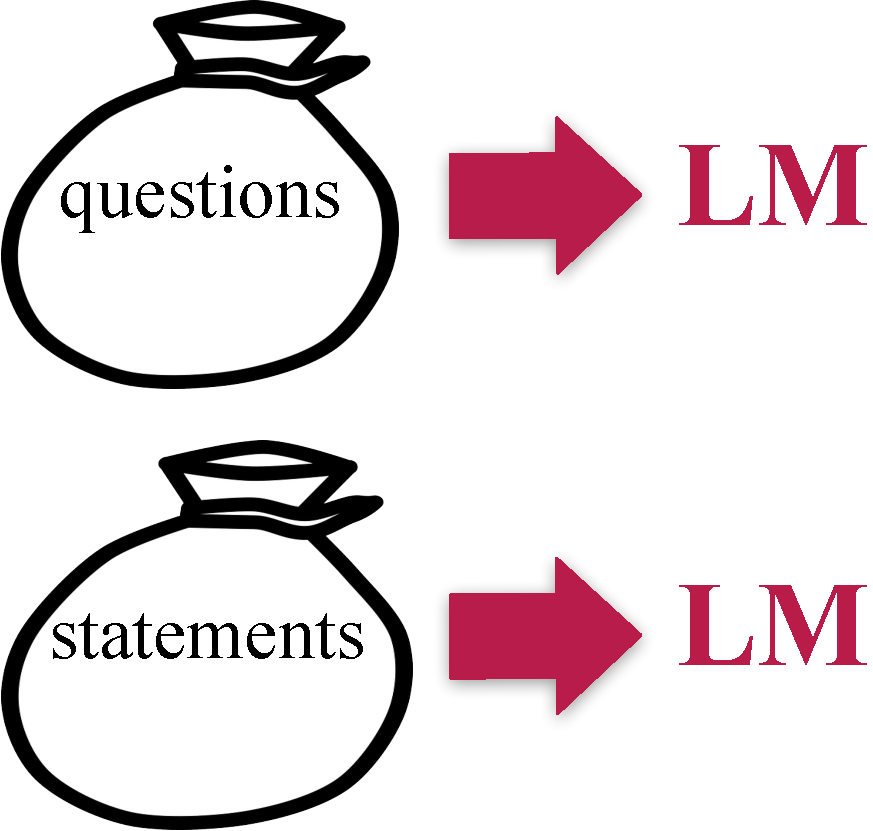
\includegraphics[scale=0.19]{Image/picture/LM-qs.pdf}
	\end{column}
	\end{columns}
\end{itemize}

\vskip5ex
\begin{center}	
	\vskip-1.3ex
	\begin{beamerboxesrounded}[width=0.85\textwidth,shadow=false]{}
	{\scriptsize

	\begin{tabular}{p{1cm}|p{7cm}}
	\multirow{2}{*}{\textbf{lexLLR}}	& we apply the \textbf{\color{purple}lexical} language models 	\\ 
						& on the \textbf{\color{purple}sequence of words}			\\
	\end{tabular}
	}
	\end{beamerboxesrounded}
\end{center}

\smallskip
\begin{center}
	\vskip-5ex
	\begin{beamerboxesrounded}[width=0.85\textwidth,shadow=false]{}
	{\scriptsize
	\begin{tabular}{p{1cm}|p{7cm}}
	 \multirow{2}{*}{\textbf{synLLR}} 	& we apply the \textbf{\color{purple}syntactic} language models	\\ 		
						& on the \textbf{\color{purple}sequence of POS tags}			\\ 
	\end{tabular}
	}
	\end{beamerboxesrounded}
\end{center}

\end{frame}

%==============================================================================================================
\begin{frame}[t]{Combined linguistic-prosodic features (3L-10P)}

\vskip-1ex
\textbf{\color{purple}Features vector}

{
\bigskip
\scriptsize
\renewcommand{\arraystretch}{1.3}
\begin{tabular}{|c|p{2.5cm}cp{6.5cm}|}
\hline
{\scriptsize \textbf{class}} 	& \multicolumn{3}{l|}{\{0=statement; 1=question\}}						\\ \hline\hline	
\parbox[t]{2mm}{\multirow{3}{*}{\rotatebox[origin=c]{90}{\scriptsize \textbf{3L}}}}
	& {lexLLR}		& = & \hskip-2ex {\scriptsize the lexical log-likelihood ratio}					\\ \cline{2-4}
	& {synLLR}		& = & \hskip-2ex {\scriptsize  the syntactic log-likelihood ratio}				\\ \cline{2-4}
	& {iP}			& = & \hskip-2ex {\scriptsize  presence or absence of interrogative pattern}			\\ \hline\hline	
\parbox[t]{2mm}{\multirow{10}{*}{\rotatebox[origin=c]{90}{\scriptsize \textbf{10P}}}}
	& {VNDurNorm}		& = & \hskip-2ex the duration of the last syllable (normalized)					\\ \cline{2-4}
	& {VNLogENorm}		& = & \hskip-2ex the logarithm of the energy of the last syllable (normalized)			\\ \cline{2-4}
	& {VNF0Delta}		& = & \hskip-2ex the F0 difference between the last syllable and the first syllable		\\ \cline{2-4}
	& {VNF0Slope}		& = & \hskip-2ex the F0 slope on the last syllable						\\ \cline{2-4}
	& {VNF0SlopeT2}		& = & \hskip-2ex VNF0Slope * VNDurNorm$^2$							\\ \cline{2-4}
	& {globalSlopeSlope}	& = & \hskip-2ex the F0 slope on the longest ending F0 slope					\\ \cline{2-4}
	& {globalSlopeLength}	& = & \hskip-2ex the length of the longest ending F0 slope					\\ \cline{2-4}
	& {globalSlopeDelta}	& = & \hskip-2ex the F0 difference between the beginning and the end of the longest ending F0 slope \\ \cline{2-4}
	& {globalSlopeSlopeT2}	& = & \hskip-2ex globalSlopeSlope * globalSlopeLength$^2$					 \\ \cline{2-4}
	& {lastF0Level}		& = & \hskip-2ex the last F0 level (normalized by speaker)					\\ \hline
         		
\end{tabular}
}


\end{frame}



%==============================================================================================================
\section{Experiments}


%==============================================================================================================
\subsection{Setups for experiments}
\begin{frame}[t]{Data for LM training}
\setcounter{framenumber}{9}

Textual corpus GigaWord

	{\scriptsize
	\begin{itemize}
	\item {\scriptsize extraction of \textbf{\color{blendedblue}statements} : sentences ending with a '.' [\#16M]}
	\item {\scriptsize extraction of \textbf{\color{blendedblue}questions} :  sentences ending with a '?' [\#89K]}
	\end{itemize}	
	}


\smallskip	
\begin{beamerboxesrounded}[width=0.85\textwidth,shadow=false]{\footnotesize word sequences}
	{\scriptsize
	\begin{tabular}{r|l}
	question	& à quel moment le raid a décidé d'intervenir?		\\ \hline
	statement	& nous sommes ensemble pour 60 minutes.			\\ 		
	\end{tabular}
	}
\end{beamerboxesrounded}

\begin{center}
	\vskip-3ex	
	$\Downarrow$
	
	\vskip-0.5ex
	{\scriptsize the \textbf{\color{purple}lexical language models} of questions and statements}
\end{center}


\smallskip
\begin{beamerboxesrounded}[width=0.90\textwidth,shadow=false]{\footnotesize part-of-speech (POS) sequence }	
{\scriptsize 
	\begin{tabular}{r|l}
	{\scriptsize question} 	& 
	    {\tiny PRP PRO$\mathalpha{:\,}$REL NOM DET$\mathalpha{:\,}$ART NOM VER$\mathalpha{:\,}$pres VER$\mathalpha{:\,}$pper PRP VER$\mathalpha{:\,}$infi }  \\ \hline
	{\scriptsize statement} & 
	    {\tiny  PRO$\mathalpha{:\,}$PER VER$\mathalpha{:\,}$pres ADV PRP NUM NOM}					\\ 		
	\end{tabular}
}
\end{beamerboxesrounded}

\begin{center}
	\vskip-3ex
	$\Downarrow$
	
	\vskip-0.5ex
	{\scriptsize the \textbf{\color{purple}syntactic language models} of questions and statements}
\end{center}


\end{frame}



%==============================================================================================================
\begin{frame}[t]{Data for training and evaluating the classifiers}

\vskip0.5cm

\begin{itemize}
\item \textbf{\color{purple}Audio corpus}: Ester, Etape, Epac 
	{\footnotesize 
	\begin{itemize}
	\vskip2ex
	\item training set : 300h of speech (manually transcribed)
	
	\vskip2ex
	\item evaluation set : 22h of speech (manually transcribed) 
	
	\vskip2ex
	\item Ester\&Epac: French broadcast news, collected from radio channels\\
			\hskip13ex (prepared speech, plus interviews)
			
	\vskip2ex
	\item Etape: debates collected from various French radio and TV channels\\
			\hskip7ex (spontaneous speech)
	\end{itemize}
	}
	
\vskip3ex
\item Data sets of \textbf{\color{purple}questions and statements} \\
	{\footnotesize \hskip5ex $\rightarrow$ sentences ending with a '?', respectively with a '.' }
\end{itemize}	


\smallskip
\begin{center}
	{\footnotesize
	\begin{tabular}{r|r|r}
			& \textbf{\#questions}	& \textbf{\#affirmations}	\\ \hline
	training 	& 10.0K			& 10.0K				\\ 
	evaluation	&  0.8K			&  7.0K				\\ 	
	\end{tabular}
	}
\end{center}

\end{frame}



%==============================================================================================================
\begin{frame}{Question / Statement classification}

\begin{itemize}
\item \textbf{\color{purple}Classifier:} the J48 decision tree (WEKA software)

\vskip4ex
\item \textbf{\color{purple}Settings}
	\begin{itemize}
	\item features extracted from manual transcriptions (0\% WER)
	
	\smallskip
	\item features extracted from automatic transcriptions (~26\% WER)
	\end{itemize}
	
\vskip4ex
\item \textbf{\color{purple}Performance}
	\begin{center}
		$\frac{1}{\text{H}}=\frac{1}{\text{2}} * \left(\frac{1}{\text{ccQuestions}}  + \frac{1}{\text{ccStatements}}\right)$
	\end{center}
	
	\vskip2ex
	{\scriptsize ccQuestions = percentage of correctly classified questions}	\\
	\vskip-0.7ex{\scriptsize ccStatements = percentage of correctly classified statements}
\end{itemize}

\vfil

\end{frame}


%==============================================================================================================
\subsection{Results}
\begin{frame}[t]{Results on prosodic features}
\setcounter{framenumber}{12}

{\footnotesize Evaluate different \textbf{\color{purple}combinations of prosodic features}}
	\vskip-0.1ex \hskip2.3ex {\color{blendedblue}$\ast$} {\scriptsize the last F0 level {\tiny \color{blendedblue} (lastF0level)}}
	\vskip-0.5ex \hskip2.3ex {\color{blendedblue}$\ast$} {\scriptsize the 5 features computed over the last syllable {\tiny \color{blendedblue} (lastSyl)}}
	\vskip-0.5ex \hskip2.3ex {\color{blendedblue}$\ast$} {\scriptsize the 5 features computed over the last syllable + the last F0 level {\tiny \color{blendedblue} (lastSyl+lastF0level)}}
	\vskip-0.5ex\hskip2.3ex {\color{blendedblue}$\ast$} {\scriptsize the 5 features computed over the ending part of the utterance {\tiny \color{blendedblue} (lastPart)}}
	\vskip-0.5ex\hskip2.3ex {\color{blendedblue}$\ast$} {\scriptsize the 6 features related to slope measurements {\tiny \color{blendedblue} (slope)}}
	\vskip-0.5ex\hskip2.3ex {\color{blendedblue}$\ast$} {\scriptsize all 10 features {\tiny \color{blendedblue} (Prosodic)}}
	
\vskip3ex
\begin{center}
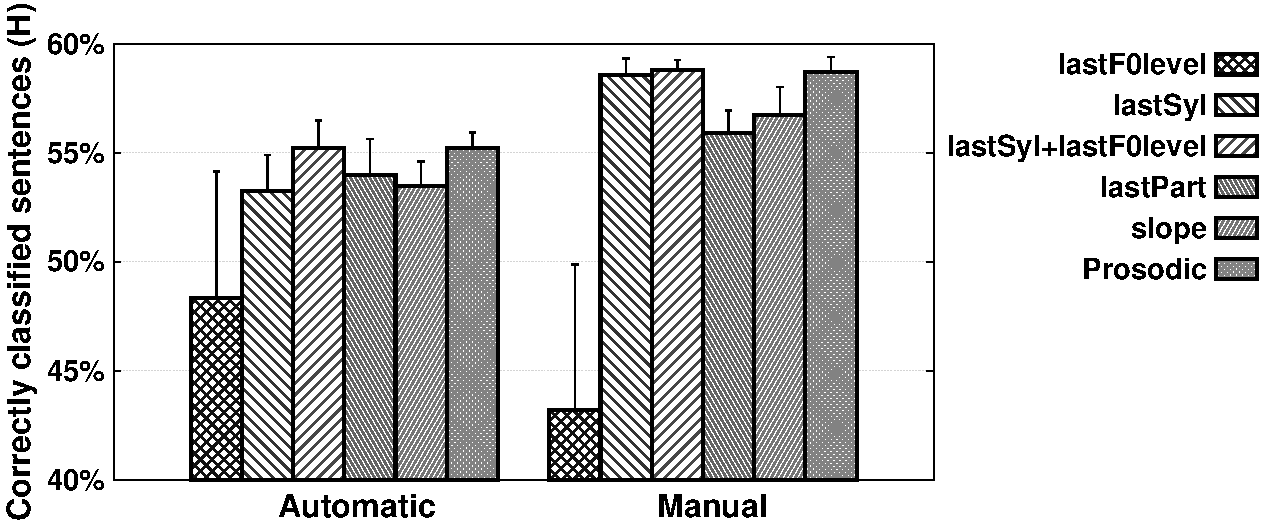
\includegraphics[scale=0.45]{Image/results/averageStats_compareProsodicFeatures_withSD.pdf}
\end{center}

\end{frame}


%==============================================================================================================
\begin{frame}[t]{Results on linguistic features}


{\footnotesize Evaluate different \textbf{\color{purple}combinations of linguistic features}}
	\vskip-0.1ex \hskip2.3ex {\color{blendedblue}$\ast$} {\scriptsize the syntactic log-likelihood ratio {\tiny \color{blendedblue} (synLLR)}}
	\vskip-0.5ex \hskip2.3ex {\color{blendedblue}$\ast$} {\scriptsize the lexical log-likelihood ratio {\tiny \color{blendedblue} (lexLLR)}}
	\vskip-0.5ex \hskip2.3ex {\color{blendedblue}$\ast$} {\scriptsize the syntactic log-likelihood ratio + the presence of interrogative patterns {\tiny \color{blendedblue} (synLLR+iP)}}\hskip-10ex \
	\vskip-0.5ex \hskip2.3ex {\color{blendedblue}$\ast$} {\scriptsize the lexical log-likelihood ratio + the presence of interrogative patterns  {\tiny \color{blendedblue} (lexLLR+iP)}}
	\vskip-0.5ex\hskip2.3ex {\color{blendedblue}$\ast$} {\scriptsize the lexical log-likelihood ratio + the syntactic log-likelihood ratio {\tiny \color{blendedblue} (lexLLR+synLLR)}}
	\vskip-0.5ex\hskip2.3ex {\color{blendedblue}$\ast$} {\scriptsize all 3 features {\tiny \color{blendedblue} (Linguistic)}}
	
\vskip3ex
\begin{center}
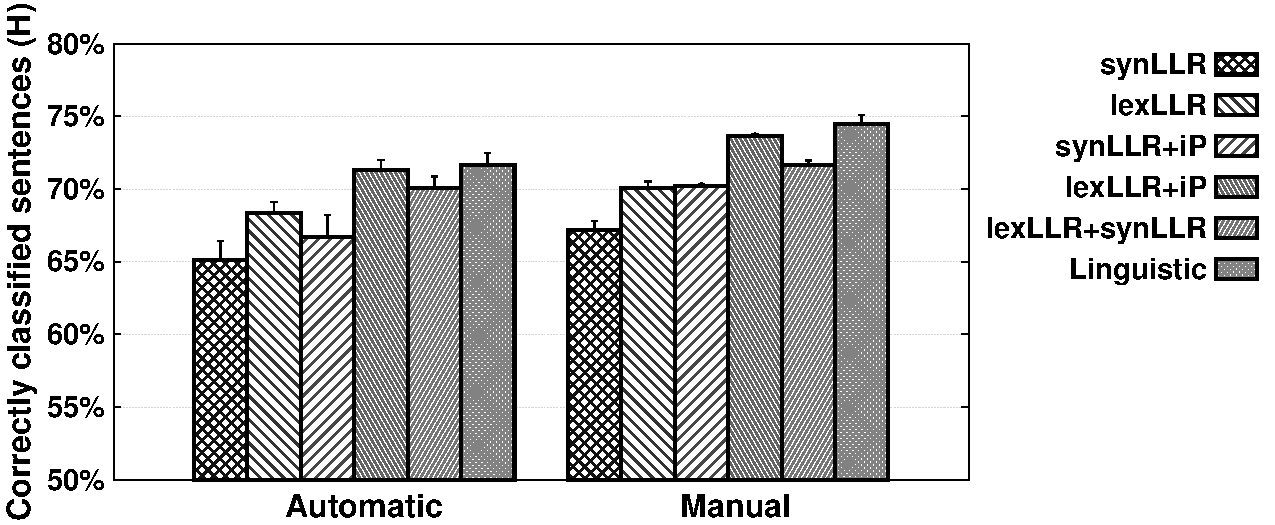
\includegraphics[scale=0.45]{Image/results/averageStats_compareLinguisticFeatures_withSD.pdf}
\end{center}

\end{frame}


%==============================================================================================================
\begin{frame}[t]{Results on prosodic, linguistic and combined features}

\vskip1ex
\begin{center}
{
Percentage of correctly classified sentences (H)
\vskip1ex

\renewcommand{\arraystretch}{1.5}
\begin{tabular}{|r|r|r|r|}
\hline
\textbf{Transcripts} 	& \textbf{Prosodic} 	& \textbf{Linguistic} 	& \textbf{Combined}	\\\hline
automatic		& 55.24\%		& 71.64\%	 	& 72.21\%		\\\hline
manual			& 58.69\%		& 74.47\%		& 74.26\%		\\\hline
\end{tabular}
}
\end{center}

{\scriptsize
\vskip4ex\hskip-5ex{\color{blendedblue}$\rightarrow$} linguistic classifier outperforms prosodic classifier
\vskip2ex\hskip-5ex{\color{blendedblue}$\rightarrow$} combined classifier outperforms linguistic classifier on automatic transcriptions
\vskip2ex\hskip-5ex{\color{blendedblue}$\rightarrow$} linguistic classifier: 3\% alsolute difference between manual and automatic transcriptions
\vskip2ex\hskip-5ex{\color{blendedblue}$\rightarrow$} combined classifier: 2\% alsolute difference between manual and automatic transcriptions
}

\end{frame}


%==============================================================================================================
\begin{frame}[t]{Best results with combined features}

\vskip5ex
\begin{center}
Confusion matrix between questions and statements \\ obtained on \textbf{\color{purple}automatic transcriptions}
\end{center}

\vskip2ex
{\footnotesize
\hskip-0.1ex
\renewcommand{\arraystretch}{1.5}
\begin{tabular}{|p{1.7cm}|p{1cm}|p{1.6cm}|p{1.6cm}|p{2cm}}
\cline{2-4}
\multicolumn{1}{c|}{}	& number 	& classified as question	& classified as statement 	& \multicolumn{1}{c}{}		\\ \cline{1-4}
question   		&  831 		& \textbf{627} 			& 204    			& \textbf{ccQuestions=75.45\%} 	\\ \cline{1-4}
statement  		& 7005 		& 1958 				& \textbf{5047}  		& \textbf{ccStatements=72.05\%} \\ \cline{1-4}
\multicolumn{4}{c}{}											& \vskip-1.5ex \textbf{\color{purple}H=73.71\%}	\\ 
\end{tabular}
}

\end{frame}


%==============================================================================================================
\begin{frame}[t]{Combine the predictions of different classifiers}

\begin{itemize}
\vskip3ex
\item use 5 different classifiers 
	\begin{itemize}
	\vskip0.2ex
	\item logistic regression 
	\vskip0.2ex
	\item J48 decision tree
	\vskip0.2ex
	\item JRip decision rules
	\vskip0.2ex
	\item sequential minimal optimization algorithm
	\vskip0.2ex
	\item multilayer perceptron 
	\end{itemize}
	
\vskip3ex
\item each classifier makes a class prediction (question / statement)

\vskip3ex
\item the final decision is made by a majority vote 
	\begin{itemize}
	\vskip2ex
	\item if at least 3 classifier assign the utterance to class "question" 
		\vskip1ex\hskip3ex {\color{blendedblue}$\rightarrow$} utterance assigned to class "question"
	\end{itemize}
	
\end{itemize}

\end{frame}

%==============================================================================================================
\begin{frame}[t]{Combine the predictions of different classifiers}

\vskip5ex

\begin{center}
Average performance obtained with all 5 classifiers \\and with their combination (by majority vote)
\end{center}

{\footnotesize
\hspace*{-4ex}
\renewcommand{\arraystretch}{1.5}
\begin{tabular}{|p{1.7cm}|p{1.1cm}|p{1.1cm}|p{1.1cm}|p{1.1cm}|p{1.1cm}|p{1.6cm}|}
\cline{2-7}
\multicolumn{1}{c|}{}	& LR		& J48		& JRip		& SMO		& MP		& combination 			\\ \hline
\textbf{Automatic}  	& 72.04  	& 72.21		& 72.81		& 69.56		& 72.07		& \vskip-3ex{\color{purple} 72.66}	\\ \hline
\textbf{Manual} 	& 73.34 	& 74.26		& 74.12		& 72.09		& 74.33		& \vskip-3ex{\color{purple} 74.91}	\\ \hline
\end{tabular}
}

\end{frame}


%==============================================================================================================
\section{Conclusions and future work}
\begin{frame}[t]{Conclusions and future work}
\setcounter{framenumber}{18}

\vskip0.4cm

\begin{itemize}
\item Conclusions 
	\vskip0.1cm
	\begin{itemize}
	\item the prosodic classifier gives poor classification results
	\vskip2ex
	\item the linguistic classifier provides by far better results \\(72\% on ASR transcripts, 74\% on manual transcripts)
	\vskip2ex
	\item the combination of prosodic and linguistic features provides a slight improvement when applied on automatic transcriptions
	\vskip2ex
	\item all 13 features are useful in detecting questions and statements
	\end{itemize}

\vskip0.3cm
\item Investigate further 
	\vskip0.1cm
	\begin{itemize}
	\item the use of confidence measures inside the classifier
	\end{itemize}
\end{itemize}


\end{frame}


%==============================================================================================================
\begin{frame}[plain]

\begin{center}
\textcolor{polyured}{\huge \textbf{Thank you \\\vskip0.2cm for your attention !}}
\end{center}

\end{frame} 



%==============================================================================================================
\begin{frame}[t,plain]{Annexe}

\begin{center}
\vskip-1ex
Confusion matrix between questions and statements
\end{center}

\vskip-1ex
{\scriptsize
\hskip-0.1ex
\begin{tabular}{|p{1.7cm}|p{1cm}|p{1.6cm}|p{1.6cm}|p{2cm}}
\cline{2-4}
\multicolumn{1}{c|}{}	& number 	& classified as question	& classified as statement 	& \multicolumn{1}{c}{}		\\ \cline{1-4}
question   		&  831 		& \textbf{627} 			& 204    			& \textbf{ccQuestions=75.45\%} 	\\ \cline{1-4}
statement  		& 7005 		& 1958 				& \textbf{5047}  		& \textbf{ccStatements=72.05\%} \\ \cline{1-4}
\multicolumn{4}{c}{}											& \vskip-1.5ex \textbf{\color{purple}H=73.71\%}	\\ 
\end{tabular}
}

{\footnotesize
\begin{itemize}
\vskip3ex
\item \textbf{\color{purple}Precision and recall on questions}

	\vskip1ex
	\begin{columns}
	\begin{column}{0.15\textwidth}			
	\end{column}
	\begin{column}{0.43\textwidth}
		\renewcommand{\arraystretch}{1.3}
		\begin{tabular}{rll}
		${\color{blendedblue}Qprecision}=$ 	& \hskip-2.1ex $\frac{627}{627+1958}=$ 	& \hskip-2ex ${\color{blendedblue}24.26\%}$ \\	
		${\color{blendedblue}Qrecall}=$ 	& \hskip-2ex $\frac{627}{627+204}=$ 	& \hskip-2ex ${\color{blendedblue}75.45\%}$ \\		
		\end{tabular}
	\end{column}
	\begin{column}{0.42\textwidth}	
		$\Rightarrow {\color{blendedblue}Qfmeasure} = {\color{blendedblue}36.72\%}$		
	\end{column}		
	\end{columns}	

\vskip4ex			
\item \textbf{\color{purple}Precision and recall on statements}

	\vskip1ex
	\begin{columns}
	\begin{column}{0.15\textwidth}			
	\end{column}
	\begin{column}{0.43\textwidth}
		\renewcommand{\arraystretch}{1.3}
		\begin{tabular}{rll}
		${\color{blendedblue}Sprecision}=$	& \hskip-2ex $\frac{5047}{5047+204}=$	& \hskip-2ex ${\color{blendedblue}96.12\%}$ \\	
		${\color{blendedblue}Srecall}=$ 	& \hskip-2ex $\frac{5047}{5047+1958}=$ 	& \hskip-2ex ${\color{blendedblue}72.05\%}$ \\		
		\end{tabular}		
	\end{column}
	\begin{column}{0.42\textwidth}	
		$\Rightarrow {\color{blendedblue}SFmeasure} = {\color{blendedblue}82.36\%}$		
	\end{column}		
	\end{columns}
	
	
	%$\frac{1}{SFmeasure}=\frac{1}{\text{2}} * \left(\frac{1}{Sprecision}  + \frac{1}{Srecall}\right) \Rightarrow {\color{blendedblue}SFmeasure} = {\color{blendedblue}82.36\%}$

\vskip4ex	
\item \textbf{\color{purple}weighted average F-measure} = {\color{blendedblue}77.52\%}
	
\end{itemize}
}

\end{frame}
%\setbeamertemplate{footline}[page number]{}
%\setbeamertemplate{footline}{}
%==============================================================================================================
%\begin{frame}{Annexe}
%\end{frame}

\end{document}


